\documentclass[12pt, a4paper]{article}

% Betöltjük a preamble.tex fájlt. Fontos a relatív elérési út!
\usepackage{booktabs}
\usepackage[T1]{fontenc}
\usepackage[utf8]{inputenc}
\usepackage[english]{babel}
\usepackage{amsmath, amssymb, amsthm} % Matek környezetek
\usepackage{geometry}
\geometry{
    a4paper,
    margin=2.5cm,
}
\usepackage{xcolor}
\usepackage{tikz}
\usepackage{float}
\usepackage{caption}
\usetikzlibrary{calc, positioning, arrows.meta, shapes.geometric, fit, matrix}

\tikzset{
    state/.style={
        matrix of nodes,
        nodes={
            draw=black!50, 
            minimum size=0.65cm, 
            anchor=center, 
            fill=white, 
            font=\ttfamily\footnotesize
        },
        column sep=-\pgflinewidth, 
        row sep=-\pgflinewidth,
        draw=black, 
        thick,
        inner sep=0pt
    },
    process/.style={rectangle, draw=black, thick, fill=white, align=center, minimum width=3.5cm, minimum height=0.8cm},
    block/.style={rectangle, draw=blue!80!black, thick, fill=blue!5, minimum width=2cm, minimum height=1cm, align=center, font=\bfseries},
    enc/.style={trapezium, trapezium angle=70, draw=black, thick, fill=gray!10, minimum width=2cm, align=center, shape border rotate=270},
    xor/.style={circle, draw=black, thick, inner sep=0pt, minimum size=0.4cm, path picture={\draw[thick] (path picture bounding box.north) -- (path picture bounding box.south) (path picture bounding box.west) -- (path picture bounding box.east);}},
    group/.style={rectangle, draw=gray, dashed, inner sep=0.3cm},
    arrow/.style={-Latex, thick},
    label/.style={font=\small\bfseries, color=gray!80!black, align=center},
    rsaStep/.style={rectangle, draw=black, thick, fill=white, align=center, minimum width=4cm, minimum height=0.8cm, rounded corners},
    data/.style={rectangle, draw=blue!80!black, thick, fill=blue!5, align=center, minimum width=2.5cm},
    arrow/.style={-Latex, thick},
    actor/.style={circle, draw=black, thick, minimum size=1.5cm, fill=gray!10, font=\bfseries},
    box/.style={rectangle, draw=black, thick, fill=white, align=center, minimum width=2.5cm, minimum height=1.5cm},
    op/.style={rectangle, draw=black, thick, fill=white, align=center, minimum width=3cm},
    decision/.style={diamond, draw=orange!80!black, thick, fill=orange!5, aspect=2, align=center, font=\small, inner sep=1pt},
    term/.style={rectangle, draw=black, thick, fill=gray!20, rounded corners, minimum height=0.8cm},
    elgamalStep/.style={rectangle, draw=black, thick, fill=white, align=center, minimum width=4cm, minimum height=0.8cm, rounded corners},
    secret/.style={rectangle, draw=red!80!black, thick, fill=red!10, align=center},
    public/.style={rectangle, draw=green!60!black, thick, fill=green!10, align=center},
    random/.style={diamond, draw=orange!80!black, thick, fill=orange!10, aspect=2, inner sep=2pt, font=\small, align=center},
    sigStep/.style={rectangle, draw=black, thick, fill=white, align=center, minimum width=4cm, minimum height=0.8cm, rounded corners},
    check/.style={diamond, draw=orange!80!black, thick, fill=orange!10, aspect=2, inner sep=2pt, font=\small, align=center},
    hash/.style={trapezium, draw=purple!80!black, thick, fill=purple!10, shape border rotate=270, align=center, minimum width=2cm}
}

\definecolor{kiemelt}{HTML}{0078A8}
\newcommand{\kiemeles}[1]{\textcolor{kiemelt}{\textbf{#1}}}

% Tételstílusok
\newtheoremstyle{tetelstilus}
    {\topsep}
    {\topsep}
    {\itshape}
    {}
    {\bfseries}
    {.}
    {.5em}
    {\thmname{#1}\thmnumber{ #2}\thmnote{ (\textbf{#3})}}
\theoremstyle{tetelstilus}

\newtheorem{defin}{Definíció}
\newtheorem{tetel}{Tétel}

\title{\LARGE\textbf{Kriptográfia}}

\usetikzlibrary{shapes, arrows, calc, positioning, intersections, patterns}


\begin{document}
\maketitle
\thispagestyle{empty} % A főcím oldalán eltávolítja az oldalszámot


\section{Geometry Pipeline}

\begin{figure}[H]  % or [!htbp] if you’re fine with floating
  \centering
  \includegraphics[width=1\textwidth]{graphics_pipeline.png} % adjust width/height as needed
\end{figure}


A grafikus szerelőszalag (pipeline) azon lépések sorozata, amelyeken keresztül a 3D-s geometriai adatok áthaladnak, míg végül 2D-s képpontokká (pixelekké) válnak a képernyőn. A modern GPU-k (Graphics Processing Unit) esetében ez a folyamat nagymértékben párhuzamosított és bizonyos szakaszai programozhatók.

A \textbf{vertex (plural: vertices)} is a point in the world. Many points are used to join the surfaces. In special cases, point clouds are drawn directly, but this is still the exception. 


\section{A programozható grafikus szerelőszalag matematikai háttere}

A grafikus csővezeték (pipeline) alapja a lineáris algebra, különösen a mátrixszorzások és a homogén koordináták használata.

\subsection{Homogén koordináták és transzformációk}
A 3D pontokat $(x, y, z)$ helyett homogén koordinátákkal $(x, y, z, w)$ ábrázoljuk (általában $w=1$). Ez lehetővé teszi, hogy az eltolást is mátrixszorzásként írjuk le.

\subsubsection{Alapvető transzformációs mátrixok}
\begin{itemize}
    \item \textbf{Eltolás (Translation):}
    $$
    T(d_x, d_y, d_z) = \begin{pmatrix} 
    1 & 0 & 0 & d_x \\ 
    0 & 1 & 0 & d_y \\ 
    0 & 0 & 1 & d_z \\ 
    0 & 0 & 0 & 1 
    \end{pmatrix}
    $$
    
    \item \textbf{Forgatás tengelyek körül (Rotation):}

    X tengely körül:
    $$
    R_x(\theta) = \begin{pmatrix} 
    1 & 0 & 0 & 0 \\ 
    0 & \cos\theta & -\sin\theta & 0 \\ 
    0 & \sin\theta & \cos\theta & 0 \\ 
    0 & 0 & 0 & 1 
    \end{pmatrix}
    $$

    Y tengely körül:
    $$
    R_y(\theta) = \begin{pmatrix} 
    \cos\theta & 0 & \sin\theta & 0 \\ 
    0 & 1 & 0 & 0 \\ 
    -\sin\theta & 0 & \cos\theta & 0 \\ 
    0 & 0 & 0 & 1 
    \end{pmatrix}
    $$

    Z tengely körül:
    $$
    R_z(\theta) = \begin{pmatrix} 
    \cos\theta & -\sin\theta & 0 & 0 \\ 
    \sin\theta & \cos\theta & 0 & 0 \\ 
    0 & 0 & 1 & 0 \\ 
    0 & 0 & 0 & 1 
    \end{pmatrix}
    $$
    
    \item \textbf{Skálázás (Scaling):}
    $$
    S(s_x, s_y, s_z) = \begin{pmatrix} 
    s_x & 0 & 0 & 0 \\ 
    0 & s_y & 0 & 0 \\ 
    0 & 0 & s_z & 0 \\ 
    0 & 0 & 0 & 1 
    \end{pmatrix}
    $$
\end{itemize}

\subsection{A koordináta-rendszerek átmenetei}
A vertex shaderben a csúcsok ($v$) a következő transzformációkon mennek keresztül:
$$ v_{clip} = M_{proj} \cdot M_{view} \cdot M_{model} \cdot v_{local} $$

\section{Inkrementális primitívrajzoló algoritmusok}

\subsection{DDA (Digital Differential Analyzer) Algoritmus}
A DDA egy egyszerű, inkrementális szakaszrajzoló eljárás. Az alapötlet a szakasz egyenletének ($y = mx + b$) deriváltjából származik. Mivel az $x$ koordinátát egységenként növeljük, az $y$ koordináta a meredekséggel ($m$) változik minden lépésben.

$$ m = \frac{y_1 - y_0}{x_1 - x_0} = \frac{\Delta y}{\Delta x} $$

\subsubsection{Algoritmus lépései (feltéve, hogy $|m| \le 1$)}
\begin{enumerate}
    \item \textbf{Inicializálás:} Kezdőpont $(x_0, y_0)$, aktuális $y = y_0$.
    \item \textbf{Ciklus} $x = x_0$-tól $x_1$-ig:
    \begin{itemize}
        \item Rajzoljuk ki a pixelt: $(x, \text{round}(y))$.
        \item $x \leftarrow x + 1$
        \item $y \leftarrow y + m$
    \end{itemize}
\end{enumerate}
\textbf{Hátránya:} Lebegőpontos műveleteket használ (összeadás és kerekítés), ami lassabb lehet az egész számos aritmetikánál, és a kerekítési hibák felhalmozódhatnak hosszú szakaszoknál.

\subsection{Bresenham Szakaszrajzoló Algoritmus}

Az algoritmus eldönti, hogy egy adott $x$ lépésnél az $y$ koordináta maradjon-e, vagy növekedjen. Az alábbi ábra szemlélteti a rácsot (pixelek) és az ideális vonalat.

\begin{center}
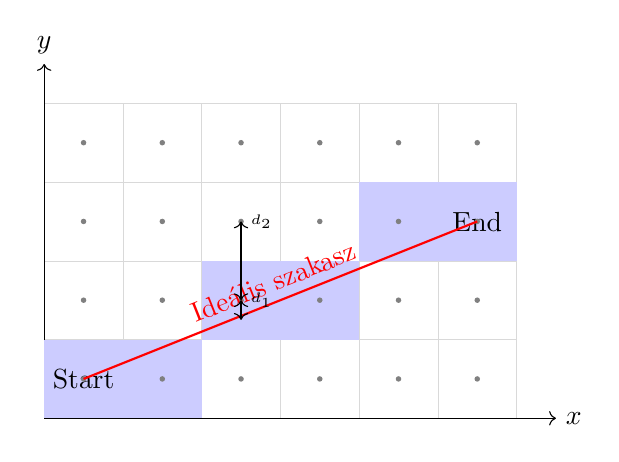
\begin{tikzpicture}[scale=1]
    % Grid
    \draw[step=1cm,gray!30,very thin] (0,0) grid (6,4);
    \draw[->] (0,0) -- (6.5,0) node[right] {$x$};
    \draw[->] (0,0) -- (0,4.5) node[above] {$y$};
    
    % Pixels (Simulated rasterization for a line with slope < 1)
    % Line from (0.5, 0.5) to (5.5, 2.5) approx
    \fill[blue!20] (0,0) rectangle (1,1); \node at (0.5,0.5) {Start};
    \fill[blue!20] (1,0) rectangle (2,1);
    \fill[blue!20] (2,1) rectangle (3,2);
    \fill[blue!20] (3,1) rectangle (4,2);
    \fill[blue!20] (4,2) rectangle (5,3);
    \fill[blue!20] (5,2) rectangle (6,3); \node at (5.5,2.5) {End};

    % Pixel centers
    \foreach \x in {0.5,1.5,...,5.5}
        \foreach \y in {0.5,1.5,...,3.5}
            \fill[gray] (\x,\y) circle (1pt);

    % Ideal line
    \draw[red, thick] (0.5,0.5) -- (5.5, 2.5) node[midway, above, sloped] {Ideális szakasz};

    % Label for d1, d2 illustration
    \draw[<->] (2.5, 1.25) -- (2.5, 1.5) node[right, font=\tiny] {$d_1$};
    \draw[<->] (2.5, 1.5) -- (2.5, 2.5) node[right, font=\tiny] {$d_2$};
    
\end{tikzpicture}
\end{center}

\textbf{A döntési változó:} $p_k = 2\Delta y \cdot x_k - 2\Delta x \cdot y_k + C$. Ez határozza meg, hogy a vonal az alsó ($d_1$) vagy felső ($d_2$) ponthoz van-e közelebb.

\subsubsection{Algoritmus lépései (Egész aritmetika)}
\begin{enumerate}
    \item \textbf{Inicializálás:} $p_0 = 2\Delta y - \Delta x$.
    \item \textbf{Ciklus} $k = 0$-tól $\Delta x - 1$-ig:
    \begin{itemize}
        \item Ha $p_k < 0 \implies (x_{k+1}, y_k)$, $p_{k+1} = p_k + 2\Delta y$.
        \item Ha $p_k \ge 0 \implies (x_{k+1}, y_k + 1)$, $p_{k+1} = p_k + 2\Delta y - 2\Delta x$.
    \end{itemize}
\end{enumerate}

\subsection{Midpoint Körrajzoló Algoritmus}
Kör egyenlete: $x^2 + y^2 - R^2 = 0$.
A döntési változó ($P_k$) a körív $(x_k+1, y_k - 1/2)$ felezőpontjának helyzetét vizsgálja.
$$ P_k = (x_k+1)^2 + (y_k - 1/2)^2 - R^2 $$

\section{Vágási algoritmusok (Clipping)}

\subsection{Cohen-Sutherland: Tartománykódok}
A vágóablak a síkot 9 részre osztja. Minden tartományhoz egy 4 bites kódot rendelünk (Outcode: Fent, Lent, Jobbra, Balra).

\begin{center}
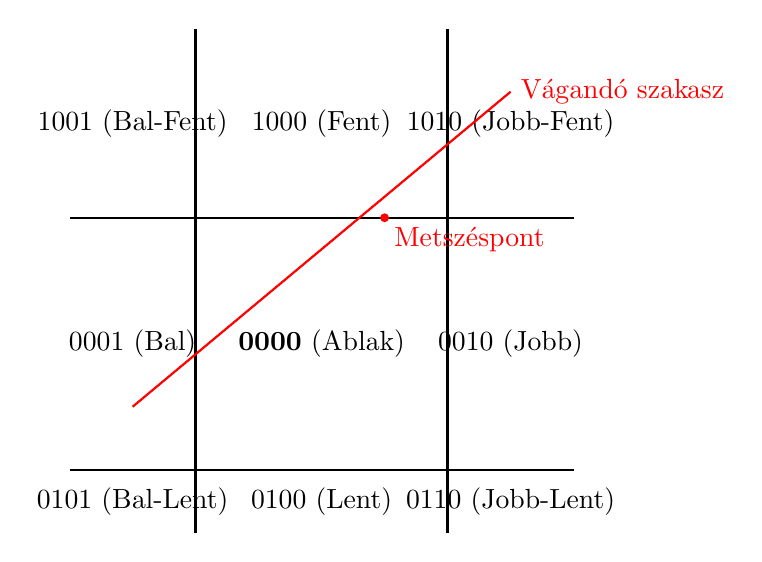
\begin{tikzpicture}[scale=0.8]
    % Lines defining regions
    \draw[thick] (-2, 2) -- (6, 2); % Upper H
    \draw[thick] (-2, -2) -- (6, -2); % Lower H
    \draw[thick] (0, -3) -- (0, 5); % Left V
    \draw[thick] (4, -3) -- (4, 5); % Right V

    % Region Codes
    \node at (2, 0) {\textbf{0000} (Ablak)};
    
    \node at (2, 3.5) {1000 (Fent)};
    \node at (2, -2.5) {0100 (Lent)};
    
    \node at (-1, 0) {0001 (Bal)};
    \node at (5, 0) {0010 (Jobb)};
    
    \node at (-1, 3.5) {1001 (Bal-Fent)};
    \node at (5, 3.5) {1010 (Jobb-Fent)};
    
    \node at (-1, -2.5) {0101 (Bal-Lent)};
    \node at (5, -2.5) {0110 (Jobb-Lent)};

    % Example Line
    \draw[red, thick] (-1, -1) -- (5, 4) node[right] {Vágandó szakasz};
    \fill[red] (3, 2) circle (2pt) node[below right] {Metszéspont};
\end{tikzpicture}
\end{center}

\textbf{Metszéspontok képletei:}
Ha $Outcode \neq 0000$, akkor metszeni kell. Például a felső szél ($y_{max}$) esetén:
$$ x = x_0 + \frac{1}{m}(y_{max} - y_0), \quad y = y_{max} $$

\subsection{Sutherland-Hodgman Poligonvágás}
Ez az algoritmus tetszőleges konvex vágóablakra (pl. téglalap) képes levágni tetszőleges poligont. A módszer lényege, hogy a poligont a vágóablak minden egyes éle mentén sorban vágjuk (pipeline-szerűen). A kimenet egy új csúcslista, amely a következő vágóél bemenete lesz.

\begin{center}
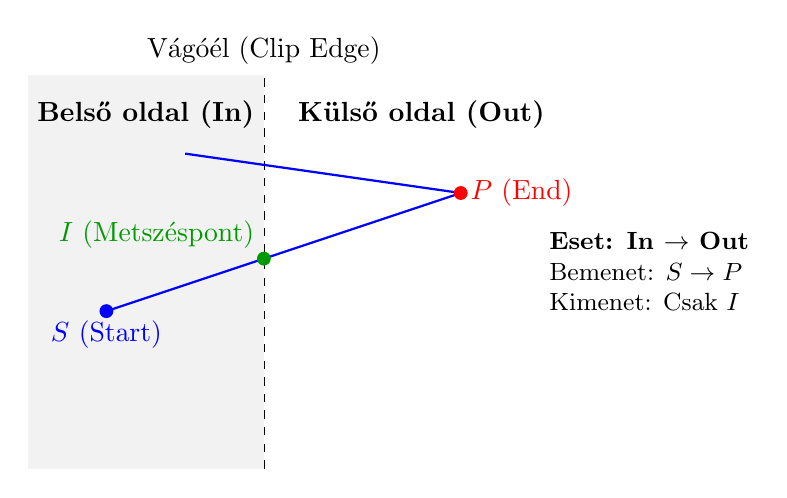
\begin{tikzpicture}[scale=1]
    % Clip edge
    \draw[thick, dashed] (0, -1) -- (0, 4) node[above] {Vágóél (Clip Edge)};
    % Fill inside
    \fill[gray!10] (-3, -1) rectangle (0, 4);
    \node at (-1.5, 3.5) {\textbf{Belső oldal (In)}};
    \node at (2, 3.5) {\textbf{Külső oldal (Out)}};

    % Polygon edges being processed
    \coordinate (V1) at (-2, 1);
    \coordinate (V2) at (2.5, 2.5); % Out
    \coordinate (V3) at (-1, 3);

    % Draw polygon outline logic
    \draw[thick, blue] (V1) -- (V2); 
    \draw[thick, blue] (V2) -- (V3);

    % Points
    \fill[blue] (V1) circle (2.5pt) node[below] {$S$ (Start)};
    \fill[red] (V2) circle (2.5pt) node[right] {$P$ (End)};
    
    % Intersections
    \path[name path=line1] (V1) -- (V2);
    \path[name path=clip] (0,-1) -- (0,4);
    \path [name intersections={of=line1 and clip,by=I1}];
    
    \fill[green!60!black] (I1) circle (2.5pt) node[above left] {$I$ (Metszéspont)};
    
    % Annotations
    \node[right, align=left, font=\small] at (3.5, 1.5) {
        \textbf{Eset: In $\to$ Out} \\
        Bemenet: $S \to P$ \\
        Kimenet: Csak $I$
    };

\end{tikzpicture}
\end{center}

\textbf{A 4 eset egy él feldolgozásakor (ahol $S$ az előző, $P$ az aktuális csúcs):}
\begin{enumerate}
    \item \textbf{In $\to$ In:} Mindkét pont belül van. $\implies$ $P$-t hozzáadjuk a kimeneti listához.
    \item \textbf{In $\to$ Out:} A szakasz kilép. $\implies$ A metszéspontot ($I$) számítjuk ki és adjuk hozzá.
    \item \textbf{Out $\to$ Out:} Mindkettő kívül van. $\implies$ Nem adunk hozzá semmit.
    \item \textbf{Out $\to$ In:} A szakasz belép. $\implies$ A metszéspontot ($I$), majd $P$-t adjuk hozzá.
\end{enumerate}

\section{Kitöltési algoritmusok}

\subsection{Pásztázó (Scan-line) algoritmus}
A sokszögkitöltés kulcsa az élek metszéspontjainak rendezése.
\begin{enumerate}
    \item \textbf{ET (Edge Table):} Élek tárolása $y_{min}$ szerint.
    \item \textbf{AET (Active Edge Table):} Az aktuális pásztázó sort metsző élek.
    \item \textbf{Párosítás:} A rendezett metszéspontok között $(x_{2i}, x_{2i+1})$ színezzük a pixeleket.
\end{enumerate}

\subsection{Él-flag (Edge-Flag) módszer}
Ez az algoritmus a kitöltést két különálló lépésben végzi a képmemóriában. Hardveresen könnyen gyorsítható.

\begin{enumerate}
    \item \textbf{1. menet (Kontúrrajzolás):} A sokszög körvonalát kirajzoljuk, de ahelyett, hogy színt írnánk a pixelbe, invertáljuk (XOR) a memóriában lévő értéket (vagy egy külön jelzőbitet). Fontos szabályok:
    \begin{itemize}
        \item A vízszintes éleket figyelmen kívül hagyjuk.
        \item A csúcspontoknál a szomszédos élek Y irányát figyeljük (lokális minimum/maximum kezelése).
    \end{itemize}
    \item \textbf{2. menet (Kitöltés):} Végigolvassuk a képernyőt (soronként, balról jobbra). Egy \textit{Inside} (Bent) logikai változót tartunk karban.
    \begin{itemize}
        \item Kezdetben $\text{Inside} = \text{False}$.
        \item Ha olyan pixelhez érünk, ahol a Flag be van állítva: $\text{Inside} = \text{!Inside}$.
        \item Ha $\text{Inside} == \text{True}$: A pixelt kiszínezzük a kitöltő színnel.
    \end{itemize}
\end{enumerate}

\begin{center}
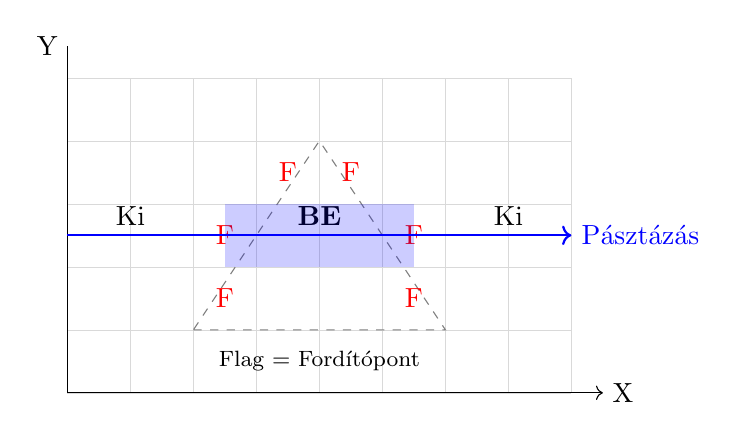
\begin{tikzpicture}[scale=0.8]
    % Grid
    \draw[step=1cm,gray!30,very thin] (0,0) grid (8,5);
    \draw[->] (0,5.5) node[left]{Y} -- (0,0) -- (8.5,0) node[right]{X};

    % Polygon Outline (Imaginary)
    \coordinate (A) at (2,1);
    \coordinate (B) at (6,1);
    \coordinate (C) at (4,4);
    \draw[dashed, gray] (A) -- (B) -- (C) -- cycle;

    % Flags (Marking the edges) - Simplified for visual
    % Left edge
    \node[red] at (2.5, 1.5) {F};
    \node[red] at (2.5, 2.5) {F};
    \node[red] at (3.5, 3.5) {F};
    
    % Right edge
    \node[red] at (5.5, 1.5) {F};
    \node[red] at (5.5, 2.5) {F};
    \node[red] at (4.5, 3.5) {F};

    % Scanline Arrow
    \draw[->, blue, thick] (0, 2.5) -- (8, 2.5) node[right] {Pásztázás};

    % Status indication
    \node[anchor=south] at (1, 2.5) {Ki};
    \node[anchor=south] at (4, 2.5) {\textbf{BE}};
    \node[anchor=south] at (7, 2.5) {Ki};
    
    % Filled area
    \fill[blue, opacity=0.2] (2.5, 2) rectangle (5.5, 3);
    \node[font=\footnotesize] at (4, 0.5) {Flag = Fordítópont};

\end{tikzpicture}
\end{center}

\section{Görbék matematikai leírása}

\subsection{Hermite-görbe (Interpoláló)}
A Hermite-görbe egy harmadfokú görbe, amelyet két végpontja ($P_1, P_4$) és a végpontokban vett érintővektorok ($R_1, R_4$) határoznak meg.

\begin{center}
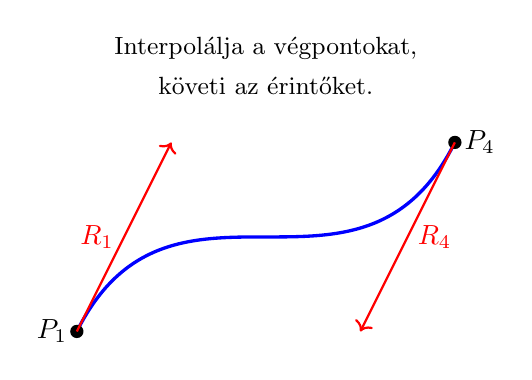
\begin{tikzpicture}[scale=1.2]
    \coordinate (P1) at (0,0);
    \coordinate (P4) at (4,2);
    
    % Draw Curve
    \draw[blue, very thick] (P1) .. controls (1,2) and (3,0) .. (P4);
    
    % Points
    \fill (P1) circle (2pt) node[left] {$P_1$};
    \fill (P4) circle (2pt) node[right] {$P_4$};
    
    % Tangents
    \draw[->, red, thick] (P1) -- (1,2) node[midway, left] {$R_1$};
    \draw[->, red, thick] (P4) -- (3,0) node[midway, right] {$R_4$};
    
    \node at (2, 3) {\small Interpolálja a végpontokat,};
    \node at (2, 2.6) {\small követi az érintőket.};
\end{tikzpicture}
\end{center}

\subsubsection{Matematikai alak (Polinom)}
A görbe egyenlete felírható a súlyfüggvények segítségével:
$$ Q(t) = H_1(t)P_1 + H_2(t)P_4 + H_3(t)R_1 + H_4(t)R_4 $$
Ahol a $H(t)$ bázisfüggvények (geometriai súlyfüggvények):
$$ H_1(t) = 2t^3 - 3t^2 + 1 \quad \text{(Kezdőpont súlya)} $$
$$ H_2(t) = -2t^3 + 3t^2 \quad \text{(Végpont súlya)} $$
$$ H_3(t) = t^3 - 2t^2 + t \quad \text{(Kezdő érintő súlya)} $$
$$ H_4(t) = t^3 - t^2 \quad \text{(Vég érintő súlya)} $$

\subsubsection{Mátrixos alak}
$$
Q(t) = \begin{pmatrix} t^3 & t^2 & t & 1 \end{pmatrix} 
\begin{pmatrix} 
2 & -2 & 1 & 1 \\ 
-3 & 3 & -2 & -1 \\ 
0 & 0 & 1 & 0 \\ 
1 & 0 & 0 & 0 
\end{pmatrix} 
\begin{pmatrix} P_1 \\ P_4 \\ R_1 \\ R_4 \end{pmatrix}
$$

\subsection{Bézier-görbék}
A harmadfokú (kubikus) Bézier-görbe 4 kontrollponttal ($P_0, P_1, P_2, P_3$) definiálható. A görbe a $P_0$-ból indul és $P_3$-ba érkezik, miközben $P_1$ és $P_2$ vonzza magához az ívet.

\begin{center}
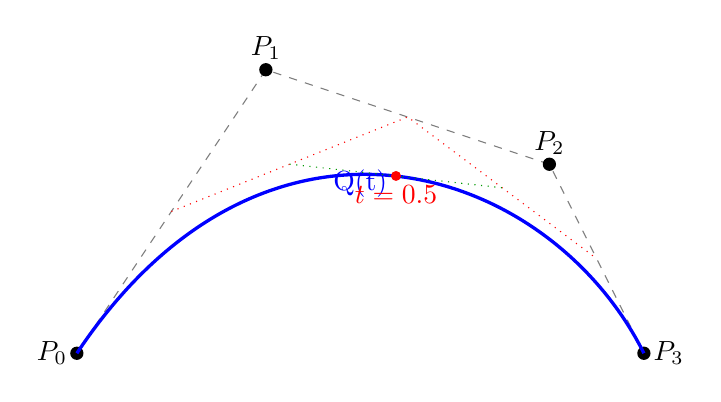
\begin{tikzpicture}[scale=1.2]
    % Control Points
    \coordinate (P0) at (0,0);
    \coordinate (P1) at (2,3);
    \coordinate (P2) at (5,2);
    \coordinate (P3) at (6,0);
    
    % Control Polygon
    \draw[dashed, gray] (P0) -- (P1) -- (P2) -- (P3);
    
    % Points
    \fill (P0) circle (2pt) node[left] {$P_0$};
    \fill (P1) circle (2pt) node[above] {$P_1$};
    \fill (P2) circle (2pt) node[above] {$P_2$};
    \fill (P3) circle (2pt) node[right] {$P_3$};
    
    % Bezier Curve
    \draw[blue, very thick] (P0) .. controls (P1) and (P2) .. (P3);
    \node[blue] at (3, 1.8) {Q(t)};

    % De Casteljau step (approx visual at t=0.5)
    \coordinate (M01) at ($(P0)!0.5!(P1)$);
    \coordinate (M12) at ($(P1)!0.5!(P2)$);
    \coordinate (M23) at ($(P2)!0.5!(P3)$);
    
    \coordinate (Q01) at ($(M01)!0.5!(M12)$);
    \coordinate (Q12) at ($(M12)!0.5!(M23)$);
    
    \coordinate (Final) at ($(Q01)!0.5!(Q12)$);
    
    \draw[dotted, red] (M01) -- (M12) -- (M23);
    \draw[dotted, green!60!black] (Q01) -- (Q12);
    \fill[red] (Final) circle (1.5pt) node[below] {$t=0.5$};
    
\end{tikzpicture}
\end{center}

\subsubsection{Matematikai alak (Bernstein-polinomok)}
A görbe általános alakja a Bernstein-polinomokkal:
$$ Q(t) = \sum_{i=0}^{3} B_{i,3}(t) P_i = (1-t)^3 P_0 + 3t(1-t)^2 P_1 + 3t^2(1-t) P_2 + t^3 P_3 $$
A súlyfüggvények tulajdonsága, hogy összegük minden $t$-re 1 (ezért marad a görbe a konvex burokban).

\subsubsection{Mátrixos alak}
$$
Q(t) = \begin{pmatrix} t^3 & t^2 & t & 1 \end{pmatrix} 
\begin{pmatrix} 
-1 & 3 & -3 & 1 \\ 
3 & -6 & 3 & 0 \\ 
-3 & 3 & 0 & 0 \\ 
1 & 0 & 0 & 0 
\end{pmatrix} 
\begin{pmatrix} P_0 \\ P_1 \\ P_2 \\ P_3 \end{pmatrix}
$$

\subsection{B-Spline görbék}
A B-Spline görbék (Basis Spline) általánosítják a Bézier-görbéket, lehetővé téve a \textbf{lokális kontrollt}. Ez azt jelenti, hogy egy kontrollpont mozgatása csak a görbe egy kis szakaszát befolyásolja. Nem feltétlenül interpolálja a végpontokat.

\subsubsection{Uniform Kubikus B-Spline}
A leggyakoribb típus a grafikában. Egy görbeszegmenst 4 kontrollpont határoz meg ($P_{i-1}, P_i, P_{i+1}, P_{i+2}$), de a görbe nem halad át egyikükön sem (hacsak nem esnek egybe). A görbék $C^2$ folytonossággal kapcsolódnak.

\begin{center}
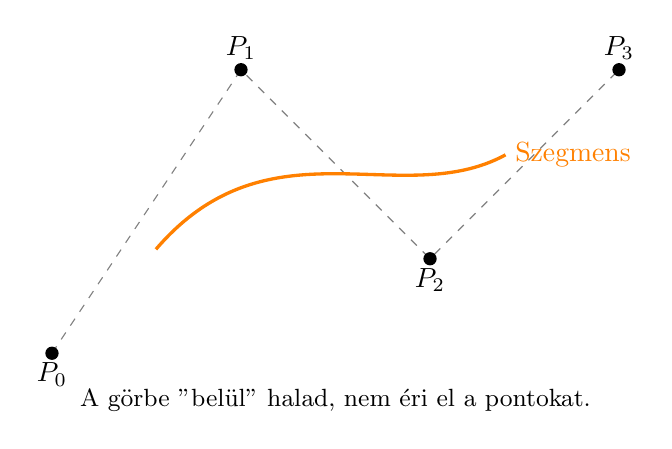
\begin{tikzpicture}[scale=1.2]
    \coordinate (P0) at (0,0);
    \coordinate (P1) at (2,3);
    \coordinate (P2) at (4,1);
    \coordinate (P3) at (6,3);
    
    \draw[dashed, gray] (P0) -- (P1) -- (P2) -- (P3);
    
    \fill (P0) circle (2pt) node[below] {$P_0$};
    \fill (P1) circle (2pt) node[above] {$P_1$};
    \fill (P2) circle (2pt) node[below] {$P_2$};
    \fill (P3) circle (2pt) node[above] {$P_3$};
    
    % Approx B-Spline segment
    \draw[orange, very thick] (1.1, 1.1) .. controls (2.3, 2.5) and (3.7, 1.5) .. (4.8, 2.1);
    
    \node[orange, right] at (4.8, 2.1) {Szegmens};
    \node at (3, -0.5) {\small A görbe "belül" halad, nem éri el a pontokat.};
\end{tikzpicture}
\end{center}

\subsubsection{Matematikai alak (Bázisfüggvények)}
A görbeszegmens egyenlete a súlyfüggvényekkel:
$$ Q_i(t) = N_0(t)P_{i-1} + N_1(t)P_i + N_2(t)P_{i+1} + N_3(t)P_{i+2} $$
Ahol a súlyfüggvények:
$$ N_0(t) = \frac{1}{6}(1-t)^3 $$
$$ N_1(t) = \frac{1}{6}(3t^3 - 6t^2 + 4) $$
$$ N_2(t) = \frac{1}{6}(-3t^3 + 3t^2 + 3t + 1) $$
$$ N_3(t) = \frac{1}{6}t^3 $$

\subsubsection{Mátrixos alak (egy szegmensre)}
$$
Q_i(t) = \frac{1}{6} \begin{pmatrix} t^3 & t^2 & t & 1 \end{pmatrix} 
\begin{pmatrix} 
-1 & 3 & -3 & 1 \\ 
3 & -6 & 3 & 0 \\ 
-3 & 0 & 3 & 0 \\ 
1 & 4 & 1 & 0 
\end{pmatrix} 
\begin{pmatrix} P_{i-1} \\ P_i \\ P_{i+1} \\ P_{i+2} \end{pmatrix}
$$

\subsubsection{Cox-de Boor formula (Általános eset)}
$$ N_{i,k}(t) = \frac{t - t_i}{t_{i+k} - t_i} N_{i,k-1}(t) + \frac{t_{i+k+1} - t}{t_{i+k+1} - t_{i+1}} N_{i+1,k-1}(t) $$


\section{Koordináta-rendszerek}

A számítógépes grafikában a geometria leírásához elengedhetetlen a megfelelő koordináta-rendszer kiválasztása.

\subsection{Descartes-féle koordináta-rendszer (Cartesian)}
Ez a legismertebb rendszer, amely egymásra merőleges tengelyekből áll ($X, Y$ síkban, $X, Y, Z$ térben).
\begin{itemize}
    \item \textbf{Bázisvektorok:} $i(1,0,0), j(0,1,0), k(0,0,1)$.
    \item \textbf{Jobbsodrású rendszer (Right-handed):} Ha a jobb kéz hüvelykujja $X$, mutatóujja $Y$, akkor a középső ujj $Z$ irányába mutat (OpenGL alapértelmezés).
    \item \textbf{Balsodrású rendszer (Left-handed):} A $Z$ tengely a képernyőbe befelé mutat (DirectX alapértelmezés).
\end{itemize}

\subsection{Baricentrikus koordináta-rendszer}
Különösen fontos a háromszögek raszterizálásánál és a sugárkövetésnél (ray tracing). Egy síkbeli pontot egy háromszög csúcspontjaihoz ($A, B, C$) viszonyítva adunk meg.

Egy $P$ pont előállítható a csúcsok súlyozott összegeként:
$$ P = \alpha A + \beta B + \gamma C $$
Ahol a súlyokra igaz, hogy:
$$ \alpha + \beta + \gamma = 1 $$
\begin{itemize}
    \item Ha $0 \le \alpha, \beta, \gamma \le 1$, akkor a pont a háromszög \textbf{belsejében} van.
    \item A koordináták arányosak a rész-háromszögek területeivel.
\end{itemize}

\subsection{Homogén koordináta-rendszer}
A projektív geometria eszköze. A síkbeli $(x, y)$ pontot $(x, y, w)$ hármassal, a térbeli $(x, y, z)$ pontot $(x, y, z, w)$ négyessel jelöljük.
\begin{itemize}
    \item Áttérés Descartes-ra: $X = x/w, Y = y/w, Z = z/w$.
    \item Ha $w=1$, az egy hagyományos pont.
    \item Ha $w=0$, az egy \textbf{irányvektor} (végtelen távoli pont).
\end{itemize}
\textbf{Jelentősége:} Lehetővé teszi, hogy az \textbf{eltolást (transzláció)} és a \textbf{perspektivikus vetítést} is mátrixszorzásként írjuk le (lineáris transzformációvá teszi az affin transzformációkat).

\section{Részletes Transzformációk: 2D és 3D Mátrixok}

Ebben a fejezetben összefoglaljuk az alapvető geometriai transzformációkat. Megkülönböztetjük a hagyományos \textbf{Descartes-i (Heterogén)} alakot (egyenletrendszerek) és a számítógépes grafikában elterjedt \textbf{Homogén} mátrixos alakot.
\\
\textit{Megjegyzés: A jelölésben oszlopvektorokat használunk ($v' = M \cdot v$).}

\subsection{Identitás (Egységmátrix)}
Ez a transzformáció nem változtatja meg a pont helyét.

\noindent\textbf{Heterogén alak:} $x' = x, \quad y' = y, \quad z' = z$.

\begin{tabular}{@{}p{0.45\textwidth}p{0.45\textwidth}@{}}
\toprule
\textbf{2D Homogén (3x3)} & \textbf{3D Homogén (4x4)} \\
\midrule
$$ I = \begin{bmatrix} 1 & 0 & 0 \\ 0 & 1 & 0 \\ 0 & 0 & 1 \end{bmatrix} $$ &
$$ I = \begin{bmatrix} 1 & 0 & 0 & 0 \\ 0 & 1 & 0 & 0 \\ 0 & 0 & 1 & 0 \\ 0 & 0 & 0 & 1 \end{bmatrix} $$ \\
\bottomrule
\end{tabular}

\subsection{Eltolás (Translation)}
Az eltolás nem lineáris transzformáció a Descartes-i térben (nem reprezentálható $2\times2$-es vagy $3\times3$-as szorzással), csak vektorösszeadással. Homogén koordinátákkal azonban mátrixszorzássá válik.
\\
\textit{Paraméterek: $d_x, d_y$ (és $d_z$ térben).}

\noindent\textbf{Heterogén alak:}
\begin{itemize}
    \item 2D: $x' = x + d_x, \quad y' = y + d_y$
    \item 3D: $x' = x + d_x, \quad y' = y + d_y, \quad z' = z + d_z$
\end{itemize}

\begin{tabular}{@{}p{0.45\textwidth}p{0.45\textwidth}@{}}
\toprule
\textbf{2D Homogén (3x3)} & \textbf{3D Homogén (4x4)} \\
\midrule
$$ T = \begin{bmatrix} 1 & 0 & d_x \\ 0 & 1 & d_y \\ 0 & 0 & 1 \end{bmatrix} $$ &
$$ T = \begin{bmatrix} 1 & 0 & 0 & d_x \\ 0 & 1 & 0 & d_y \\ 0 & 0 & 1 & d_z \\ 0 & 0 & 0 & 1 \end{bmatrix} $$ \\
\bottomrule
\end{tabular}

\subsection{Méretezés / Skálázás (Scaling)}
A tengelyek mentén történő nyújtás vagy zsugorítás. Ha $s_x = s_y (= s_z)$, akkor egyenletes (hasonlósági) skálázásról beszélünk.
\\
\textit{Paraméterek: $s_x, s_y$ (és $s_z$).}

\noindent\textbf{Heterogén alak:}
\begin{itemize}
    \item 2D: $x' = x \cdot s_x, \quad y' = y \cdot s_y$
    \item 3D: $x' = x \cdot s_x, \quad y' = y \cdot s_y, \quad z' = z \cdot s_z$
\end{itemize}

\begin{tabular}{@{}p{0.45\textwidth}p{0.45\textwidth}@{}}
\toprule
\textbf{2D Homogén (3x3)} & \textbf{3D Homogén (4x4)} \\
\midrule
$$ S = \begin{bmatrix} s_x & 0 & 0 \\ 0 & s_y & 0 \\ 0 & 0 & 1 \end{bmatrix} $$ &
$$ S = \begin{bmatrix} s_x & 0 & 0 & 0 \\ 0 & s_y & 0 & 0 \\ 0 & 0 & s_z & 0 \\ 0 & 0 & 0 & 1 \end{bmatrix} $$ \\
\bottomrule
\end{tabular}

\subsection{Forgatás (Rotation)}
A forgatás az origó (vagy térben egy tengely) körül történik $\alpha$ szöggel. Pozitív szög esetén az óramutató járásával ellentétes irányba.

\subsubsection{2D Forgatás (Origó körül)}
\textbf{Heterogén alak:}
$$ x' = x \cos \alpha - y \sin \alpha $$
$$ y' = x \sin \alpha + y \cos \alpha $$

\textbf{Homogén (3x3):}
$$ R(\alpha) = \begin{bmatrix} \cos \alpha & -\sin \alpha & 0 \\ \sin \alpha & \cos \alpha & 0 \\ 0 & 0 & 1 \end{bmatrix} $$

\subsubsection{3D Forgatás (Főtengelyek körül)}
Térben 4x4-es mátrixokat használunk.

\begin{itemize}
    \item \textbf{Z-tengely körül (síkforgatás kiterjesztése):}
    \\ \textit{Heterogén:} $x' = x \cos \alpha - y \sin \alpha, \quad y' = x \sin \alpha + y \cos \alpha, \quad z' = z$
    $$ R_z(\alpha) = \begin{bmatrix} \cos \alpha & -\sin \alpha & 0 & 0 \\ \sin \alpha & \cos \alpha & 0 & 0 \\ 0 & 0 & 1 & 0 \\ 0 & 0 & 0 & 1 \end{bmatrix} $$
    
    \item \textbf{X-tengely körül:}
    \\ \textit{Heterogén:} $y' = y \cos \alpha - z \sin \alpha, \quad z' = y \sin \alpha + z \cos \alpha, \quad x' = x$
    $$ R_x(\alpha) = \begin{bmatrix} 1 & 0 & 0 & 0 \\ 0 & \cos \alpha & -\sin \alpha & 0 \\ 0 & \sin \alpha & \cos \alpha & 0 \\ 0 & 0 & 0 & 1 \end{bmatrix} $$
    
    \item \textbf{Y-tengely körül:}
    \\ \textit{Heterogén:} $z' = z \cos \alpha - x \sin \alpha, \quad x' = z \sin \alpha + x \cos \alpha, \quad y' = y$
    $$ R_y(\alpha) = \begin{bmatrix} \cos \alpha & 0 & \sin \alpha & 0 \\ 0 & 1 & 0 & 0 \\ -\sin \alpha & 0 & \cos \alpha & 0 \\ 0 & 0 & 0 & 1 \end{bmatrix} $$
\end{itemize}

\subsection{Tükrözés (Reflection)}
A tükrözés speciális skálázásnak is felfogható, ahol a skálázási tényező $-1$. A determináns értéke $-1$.

\begin{tabular}{@{}p{0.45\textwidth}p{0.45\textwidth}@{}}
\toprule
\textbf{2D Tükrözés (Tengelyekre)} & \textbf{3D Tükrözés (Síkokra)} \\
\midrule
X-tengelyre ($y \to -y$): & XY síkra ($z \to -z$): \\
\textit{Heterogén:} $x' = x, y' = -y$ & \textit{Heterogén:} $x'=x, y'=y, z'=-z$ \\
$$ M_x = \begin{bmatrix} 1 & 0 & 0 \\ 0 & -1 & 0 \\ 0 & 0 & 1 \end{bmatrix} $$ &
$$ M_{xy} = \begin{bmatrix} 1 & 0 & 0 & 0 \\ 0 & 1 & 0 & 0 \\ 0 & 0 & -1 & 0 \\ 0 & 0 & 0 & 1 \end{bmatrix} $$ \\
\vspace{0.1cm}
Origóra ($x \to -x, y \to -y$): & Origóra: \\
\textit{Heterogén:} $x' = -x, y' = -y$ & \textit{Heterogén:} $x'=-x, y'=-y, z'=-z$ \\
$$ M_o = \begin{bmatrix} -1 & 0 & 0 \\ 0 & -1 & 0 \\ 0 & 0 & 1 \end{bmatrix} $$ &
$$ M_o = \begin{bmatrix} -1 & 0 & 0 & 0 \\ 0 & -1 & 0 & 0 \\ 0 & 0 & -1 & 0 \\ 0 & 0 & 0 & 1 \end{bmatrix} $$ \\
\bottomrule
\end{tabular}

\subsection{Nyírás (Shearing)}
A nyírás során az egyik koordináta értéke függ egy másik koordinátától. Affin transzformáció, párhuzamosságot megőriz, de a szögeket és távolságokat nem.

\subsubsection{2D Nyírás}
X-irányú nyírás (az X koordináta változik Y függvényében):
\\ \textbf{Heterogén:} $x' = x + sh_x \cdot y, \quad y' = y$.
$$ Sh_x = \begin{bmatrix} 1 & sh_x & 0 \\ 0 & 1 & 0 \\ 0 & 0 & 1 \end{bmatrix} $$
Y-irányú nyírás:
\\ \textbf{Heterogén:} $x' = x, \quad y' = y + sh_y \cdot x$.
$$ Sh_y = \begin{bmatrix} 1 & 0 & 0 \\ sh_y & 1 & 0 \\ 0 & 0 & 1 \end{bmatrix} $$

\subsubsection{3D Nyírás}
Itt több lehetőség van. Például, ha a Z koordinátát nem változtatjuk, de X-et és Y-t a Z függvényében nyírjuk:
\\ \textbf{Heterogén:} $x' = x + sh_x \cdot z, \quad y' = y + sh_y \cdot z, \quad z' = z$.
$$ H_{xy(z)} = \begin{bmatrix} 1 & 0 & sh_{x} & 0 \\ 0 & 1 & sh_{y} & 0 \\ 0 & 0 & 1 & 0 \\ 0 & 0 & 0 & 1 \end{bmatrix} $$

\section{Transzformációk osztályozása és szorzata}

A geometriai transzformációkat aszerint csoportosítjuk, hogy milyen invariánsokat (változatlan tulajdonságokat) őriznek meg.

\subsection{Osztályozás (Klein-féle program szerint)}

\begin{enumerate}
    \item \textbf{Egybevágósági transzformációk (Izometriák):}
    \begin{itemize}
        \item Megőrzi: Távolságot, szögeket, területeket.
        \item Példa: Eltolás, Forgatás, Tükrözés.
        \item Mátrix alak: $\det(M) = \pm 1$ (ortogonális rész).
    \end{itemize}

    \item \textbf{Hasonlósági transzformációk:}
    \begin{itemize}
        \item Megőrzi: Szögeket, távolságok \textit{arányát}.
        \item Példa: Egyenletes skálázás ($s_x = s_y = s_z$).
    \end{itemize}

    \item \textbf{Affin transzformációk:}
    \begin{itemize}
        \item Megőrzi: Párhuzamosságot, osztóviszonyt (szakaszok arányát egy egyenesen).
        \item Példa: Nyírás (Shearing), nem egyenletes skálázás.
        \item Mátrix alakja: Az utolsó sor mindig $[0, 0, 0, 1]$.
        $$
        M_{affin} = \begin{bmatrix} A & t \\ 0^T & 1 \end{bmatrix}
        $$
        ahol $A$ a lineáris rész (3x3), $t$ az eltolás.
    \end{itemize}

    \item \textbf{Projektív transzformációk:}
    \begin{itemize}
        \item Megőrzi: Egyenest (egyenes képe egyenes), illeszkedést.
        \item \textbf{NEM} őrzi meg a párhuzamosságot (enyészpontok keletkeznek).
        \item Mátrix alakja: Az utolsó sor bármi lehet. Ez felelős a perspektív torzításért.
    \end{itemize}
\end{enumerate}

\subsection{Transzformációk szorzata}
Több transzformáció egymásutánja egyetlen mátrixszal helyettesíthető.
$$ v' = M_n \cdot M_{n-1} \cdot \dots \cdot M_2 \cdot M_1 \cdot v $$
$$ M_{eredő} = M_n \cdot \dots \cdot M_1 $$
\textbf{Fontos:} A mátrixszorzás \textbf{nem kommutatív}! ($A \cdot B \neq B \cdot A$).
Például: Nem mindegy, hogy előbb forgatunk és utána toljuk el a koordinátarendszert, vagy fordítva.

\section{Koordináta-transzformációk}

Kétféleképpen értelmezhetjük a transzformációkat:
\begin{enumerate}
    \item \textbf{Ponttranszformáció:} A koordinátarendszer rögzített, az objektum pontjai mozognak benne.
    \item \textbf{Koordináta-transzformáció (Báziscsere):} A pont a térben rögzített, de a koordinátarendszert (bázist) mozgatjuk alatta, így a pont koordinátái megváltoznak.
\end{enumerate}

Ha egy $K_1$ rendszerből áttérünk egy $K_2$-be, és a $K_2$ rendszer origója és bázisvektorai $K_1$-ben kifejezve $M$ mátrixszal írhatók le (ahol az oszlopok az új bázisvektorok), akkor a pont új koordinátái:
$$ v_{K2} = M^{-1} \cdot v_{K1} $$
Tehát a koordináta-transzformáció mátrixa az objektum-transzformáció mátrixának az inverze.

\begin{center}
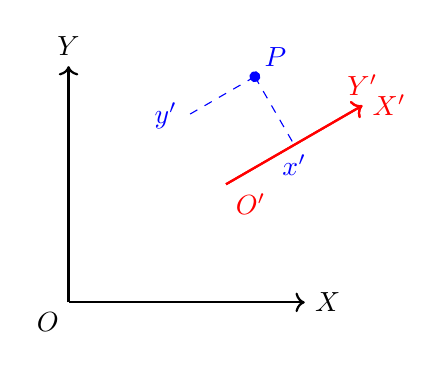
\begin{tikzpicture}[scale=1]
    % Global system
    \draw[->, thick] (0,0) -- (3,0) node[right] {$X$};
    \draw[->, thick] (0,0) -- (0,3) node[above] {$Y$};
    \node at (0,0) [below left] {$O$};

    % Local System (Rotated and Translated)
    \begin{scope}[shift={(2,1.5)}, rotate=30]
        \draw[->, thick, red] (0,0) -- (2,0) node[right] {$X'$};
        \draw[->, thick, red] (0,0) -- (2,0) node[above] {$Y'$};
        \node at (0,0) [below right, red] {$O'$};
        
        \fill[blue] (1,1) circle (2pt) node[above right] {$P$};
        \draw[dashed, blue] (1,1) -- (1,0) node[below] {$x'$};
        \draw[dashed, blue] (1,1) -- (0,1) node[left] {$y'$};
    \end{scope}
\end{tikzpicture}
\end{center}

\section{Tér leképezése síkra (Viewing Pipeline)}

A 3D színtér síkra vetítése több lépésből áll:
$$ P_{screen} = M_{viewport} \cdot M_{proj} \cdot M_{view} \cdot M_{model} \cdot P_{local} $$

\subsection{Viewing Transzformáció (Nézeti transzformáció)}
A transzformáció célja, hogy a világkoordinátákat $(P_{world})$ átalakítsa a kamera koordinátarendszerébe $(P_{view})$. Ez technikailag a kamera mozgatásának inverze: ha a kamerát $+10$-zel toljuk $Z$-ben, az egyenértékű azzal, ha a világot $-10$-zel toljuk $Z$-ben.

\subsubsection{Matematikai levezetés (Báziscsere)}
Adott a kamera három paramétere (LookAt függvény):
\begin{itemize}
    \item $E$ (Eye): A kamera pozíciója (Origó lesz az új rendszerben).
    \item $C$ (Center/Target): A pont, ahova a kamera néz.
    \item $U$ (Up): A "felfelé" mutató irány (közelítőleg).
\end{itemize}

Az új koordinátarendszer ($u, v, n$ bázisvektorok) kiszámítása (Jobbsodrású rendszer, kamera $-Z$ felé néz):

\begin{enumerate}
    \item \textbf{Előre vektor ($n$ vagy $Z_{axis}$):} A kamera $-Z$ irányba néz, tehát a $+Z$ irány a kamerától kifelé mutat (hátra).
    $$ n = \frac{E - C}{||E - C||} $$
    \item \textbf{Jobbra vektor ($u$ vagy $X_{axis}$):} Az Up vektor és az $n$ vektor keresztszorzata.
    $$ u = \frac{U \times n}{||U \times n||} $$
    \item \textbf{Fel vektor ($v$ vagy $Y_{axis}$):} A korrigált felfelé irány (hogy a bázis ortogonális legyen).
    $$ v = n \times u $$
\end{enumerate}

\subsubsection{A Mátrix felépítése}
A Viewing mátrix ($M_{view}$) két transzformációból áll: egy eltolásból ($T$), amely a kamera pozícióját ($E$) az origóba viszi, és egy forgatásból ($R$), amely a világ bázisát a kamera bázisába ($u, v, n$) forgatja. Mivel koordináta-rendszer transzformációról van szó (inverz), a forgatási mátrix sorai az új bázisvektorok lesznek.

$$ M_{view} = R \cdot T $$

$$ T = \begin{bmatrix} 1 & 0 & 0 & -E_x \\ 0 & 1 & 0 & -E_y \\ 0 & 0 & 1 & -E_z \\ 0 & 0 & 0 & 1 \end{bmatrix} \quad \text{és} \quad R = \begin{bmatrix} u_x & u_y & u_z & 0 \\ v_x & v_y & v_z & 0 \\ n_x & n_y & n_z & 0 \\ 0 & 0 & 0 & 1 \end{bmatrix} $$

$$ M_{view} = \begin{bmatrix} u_x & u_y & u_z & -(u \cdot E) \\ v_x & v_y & v_z & -(v \cdot E) \\ n_x & n_y & n_z & -(n \cdot E) \\ 0 & 0 & 0 & 1 \end{bmatrix} $$

\subsubsection{Számítási Példa}
Legyen $E = (0, 0, 5)$ (Kamera a Z-tengelyen), $C = (0, 0, 0)$ (Origóba néz), $U = (0, 1, 0)$.

1. $n = (0, 0, 5) - (0, 0, 0) = (0, 0, 5) \to \text{Normálva: } (0, 0, 1)$.
2. $u = (0, 1, 0) \times (0, 0, 1) = (1, 0, 0)$.
3. $v = (0, 0, 1) \times (1, 0, 0) = (0, 1, 0)$.

Mátrix összeállítása:
$$ -u \cdot E = -(1\cdot0 + 0\cdot0 + 0\cdot5) = 0 $$
$$ -v \cdot E = -(0\cdot0 + 1\cdot0 + 0\cdot5) = 0 $$
$$ -n \cdot E = -(0\cdot0 + 0\cdot0 + 1\cdot5) = -5 $$

$$ M_{view} = \begin{bmatrix} 1 & 0 & 0 & 0 \\ 0 & 1 & 0 & 0 \\ 0 & 0 & 1 & -5 \\ 0 & 0 & 0 & 1 \end{bmatrix} $$
Ez megfelel annak, hogy a világot 5 egységgel eltoljuk a $-Z$ irányba (a kamera elé).

\subsection{Vetítések (Projection)}

\subsubsection{Párhuzamos (Ortografikus) vetítés}
A vetítési sugarak párhuzamosak. Megőrzi a méreteket, függetlenül a távolságtól (mérnöki ábrázolás).
Mátrixa egyszerűen skálázza és eltolja a koordinátákat a $[-1, 1]$ kockába (NDC).

\subsubsection{Perspektív vetítés}
A vetítési sugarak egy közös pontba (szem/kamera) futnak össze. A távolabbi tárgyak kisebbnek látszanak.
Ez a $w$ koordinátával történő osztással érhető el (perspektivikus osztás).

A vetítési mátrix egyszerűsített alakja (ahol $d$ a fókusztávolság):
$$
M_{persp} = \begin{bmatrix}
1 & 0 & 0 & 0 \\
0 & 1 & 0 & 0 \\
0 & 0 & 1 & 0 \\
0 & 0 & 1/d & 0
\end{bmatrix}
$$
Ekkor a homogén koordináta: $P(x, y, z, z/d)$.
Az osztás után: $P'( \frac{x}{z/d}, \frac{y}{z/d}, d )$. Tehát az $x'$ és $y'$ koordináták fordítottan arányosak $z$-vel.

\begin{center}
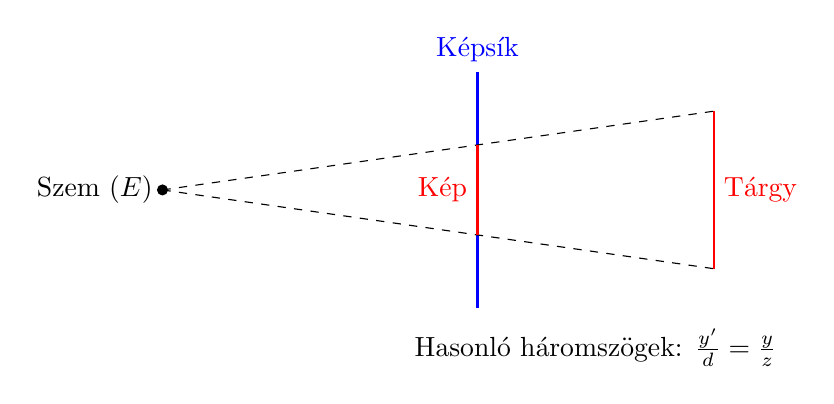
\begin{tikzpicture}[scale=1]
    % Eye
    \coordinate (Eye) at (-4, 1.5);
    \fill (Eye) circle (2pt) node[left] {Szem ($E$)};

    % Image Plane
    \draw[thick, blue] (0, 0) -- (0, 3) node[above] {Képsík};

    % Object
    \coordinate (P1) at (3, 0.5);
    \coordinate (P2) at (3, 2.5);
    \draw[thick, red] (P1) -- (P2) node[midway, right] {Tárgy};

    % Rays
    \draw[dashed] (Eye) -- (P1);
    \draw[dashed] (Eye) -- (P2);

    % Projections
    \coordinate (Proj1) at (intersection of Eye--P1 and 0,0--0,3);
    \coordinate (Proj2) at (intersection of Eye--P2 and 0,0--0,3);
    
    \draw[thick, red] (Proj1) -- (Proj2) node[midway, left] {Kép};
    
    \node at (1.5, -0.5) {Hasonló háromszögek: $\frac{y'}{d} = \frac{y}{z}$};
\end{tikzpicture}
\end{center}


\section{Felületreprezentációs módszerek}

A 3D-s objektumok felületének leírására többféle matematikai megközelítés létezik, amelyek eltérő alkalmazásokban előnyösek.

\subsection{Explicit reprezentáció}
A felületet egy függvényként adjuk meg, ahol az egyik koordináta a másik kettő függvénye.
$$ y = f(x, z) $$
\begin{itemize}
    \item \textbf{Normálvektor számítása:} A felület érintősíkjának normálisa a parciális deriváltakból számolható.
    $$ n = \left( -\frac{\partial f}{\partial x}, 1, -\frac{\partial f}{\partial z} \right) $$
    \item \textbf{Hátránya:} Nem képes zárt alakzatokat (pl. gömb) leírni.
\end{itemize}

\subsection{Implicit reprezentáció}
A felületet egy egyenlet megoldáshalmazaként definiáljuk: $F(x, y, z) = 0$.
Példa (Gömb): $x^2 + y^2 + z^2 - R^2 = 0$.

\subsubsection{Matematikai háttér: A Gradiens}
Az implicit felületek legfontosabb tulajdonsága, hogy a felület normálvektora ($N$) bármely $P(x,y,z)$ pontban megegyezik a függvény gradiensvektorával ($\nabla F$) abban a pontban.
$$ N(x, y, z) = \nabla F = \begin{pmatrix} \frac{\partial F}{\partial x} \\ \frac{\partial F}{\partial y} \\ \frac{\partial F}{\partial z} \end{pmatrix} $$
Példa: Gömb esetén $N = (2x, 2y, 2z)$, ami (normalizálva) valóban a középpontból kifelé mutató vektor.

\subsection{Paraméteres felületek}
A felület pontjait két paraméter ($u, v$) függvényében adjuk meg:
$$ P(u, v) = \begin{pmatrix} x(u, v) \\ y(u, v) \\ z(u, v) \end{pmatrix}, \quad u, v \in [0, 1] $$

\begin{center}
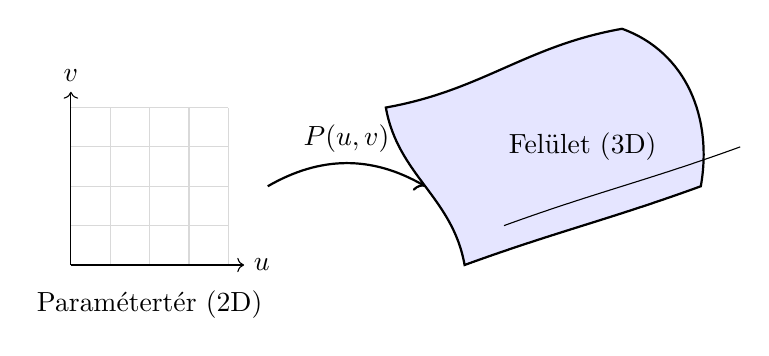
\begin{tikzpicture}
    % UV space
    \draw[step=0.5, gray!30] (0,0) grid (2,2);
    \draw[->] (0,0) -- (2.2,0) node[right] {$u$};
    \draw[->] (0,0) -- (0,2.2) node[above] {$v$};
    \node at (1, -0.5) {Paramétertér (2D)};

    % Arrow
    \draw[->, thick, bend left] (2.5, 1) to node[above] {$P(u,v)$} (4.5, 1);

    % 3D Surface
    \begin{scope}[shift={(5,0)}]
        \draw[thick, fill=blue!10] (0,0) to[out=20,in=200] (3,1) to[out=80,in=-20] (2,3) to[out=190,in=10] (-1,2) to[out=-80,in=100] cycle;
        \draw[thin] (0,0) to[out=20,in=200] (3,1); % u curve
        \draw[thin] (0.5,0.5) to[out=20,in=200] (3.5,1.5); % u curve
        \draw[thin] (-1,2) to[out=-80,in=100] (0,0); % v curve
        \node at (1.5, 1.5) {Felület (3D)};
    \end{scope}
\end{tikzpicture}
\end{center}

\subsubsection{Differenciálgeometria: Érintők és Normális}
A felületi normálvektor a két érintővektor vektoriális szorzata:
$$ N(u, v) = \frac{T_u \times T_v}{||T_u \times T_v||}, \quad \text{ahol } T_u = \frac{\partial P}{\partial u}, T_v = \frac{\partial P}{\partial v} $$

\subsection{Bikubikus felületek (Bézier-felületek)}
A Bézier-felületet 16 darab kontrollpont ($P_{00} \dots P_{33}$) határozza meg. A felület "kifeszül" ezen pontok közé.

\begin{center}
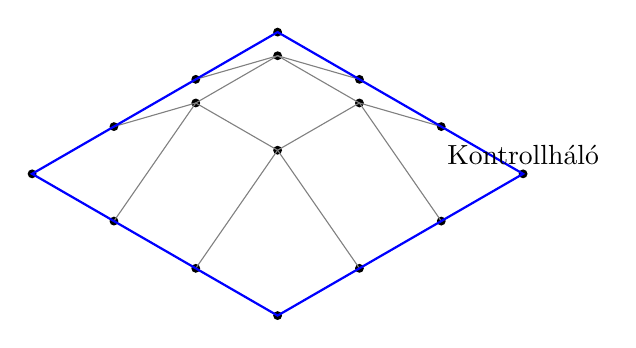
\begin{tikzpicture}[scale=0.8, x={(0.866cm,-0.5cm)}, y={(0.866cm,0.5cm)}, z={(0cm,1cm)}]
    % Control Points 4x4 grid
    \foreach \x in {0,1,2,3} {
        \foreach \y in {0,1,2,3} {
             % Create some curvature
             \pgfmathsetmacro{\z}{sin(\x*60)*sin(\y*60)*1.5}
             \coordinate (P\x\y) at (\x*1.5, \y*1.5, \z);
             \fill (P\x\y) circle (2pt);
        }
    }
    
    % Draw lines u-direction
    \foreach \y in {0,1,2,3} {
        \draw[gray] (P0\y) -- (P1\y) -- (P2\y) -- (P3\y);
    }
    % Draw lines v-direction
    \foreach \x in {0,1,2,3} {
        \draw[gray] (P\x0) -- (P\x1) -- (P\x2) -- (P\x3);
    }
    
    % Surface approximation (just edges)
    \draw[thick, blue] (P00) -- (P10) -- (P20) -- (P30) -- (P31) -- (P32) -- (P33) -- (P23) -- (P13) -- (P03) -- (P02) -- (P01) -- cycle;
    
    \node[anchor=south] at (P33) {Kontrollháló};
\end{tikzpicture}
\end{center}

A mátrixos egyenlet:
$$ Q(u, v) = U \cdot M \cdot G \cdot M^T \cdot V^T $$

\subsubsection{Bézier-felület normálvektora}
A fényeléshez szükségünk van a normálvektorra. Ehhez deriválnunk kell a $Q(u, v)$ függvényt $u$ és $v$ szerint.
$$ N = \frac{\partial Q}{\partial u} \times \frac{\partial Q}{\partial v} $$

\section{Felület leíró adatstruktúrák}
(A korábbi leírás változatlan: Csúcslista, Laplista, Winged-Edge).

\section{Láthatósági algoritmusok}

\subsection{Hátsó lap eldobás (Backface Culling)}
Zárt testeknél a hátsó lapok eldobhatók.

\begin{center}
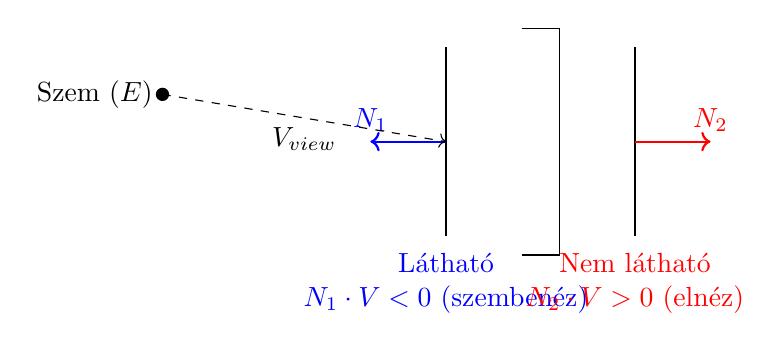
\begin{tikzpicture}[scale=1.2]
    \coordinate (Eye) at (-3,0.5);
    \fill (Eye) circle (2pt) node[left] {Szem ($E$)};
    
    % Object
    \coordinate (Center) at (1,0);
    
    % Front Face
    \draw[thick] (0, 1) -- (0, -1);
    \draw[->, blue, thick] (0,0) -- (-0.8, 0) node[above] {$N_1$};
    \draw[->, dashed] (Eye) -- (0,0) node[midway, below] {$V_{view}$};
    
    % Back Face
    \draw[thick] (2, 1) -- (2, -1);
    \draw[->, red, thick] (2,0) -- (2.8, 0) node[above] {$N_2$};
    
    \node[blue, align=center] at (0, -1.5) {Látható\\$N_1 \cdot V < 0$ (szembenéz)};
    \node[red, align=center] at (2, -1.5) {Nem látható\\$N_2 \cdot V > 0$ (elnéz)};
    
    \draw (0.8, 1.2) -- (1.2, 1.2) -- (1.2, -1.2) -- (0.8, -1.2); % Indicating it's a closed object
\end{tikzpicture}
\end{center}

$$ \cos \theta = \frac{N \cdot V}{||N|| \cdot ||V||} $$

\subsection{Z-buffer (Mélységi puffer)}
A perspektivikus vetítés során a $z$ koordináták nem lineárisan képeződnek le. A Z-bufferben tárolt érték ($z'$) és a valós távolság ($z_{eye}$) közötti kapcsolat:
$$ z' = \frac{a}{z_{eye}} + b $$

\section{Fény- és anyagtulajdonságok}
(A korábbi leírás változatlan: Ambient, Diffuse, Specular komponensek).

\section{Megvilágítási és árnyalási modellek - Matematikai Mélységek}

\subsection{Lambert-féle koszinusz törvény (Diffuse)}
A matt felületek fényvisszaverése a beesési szög koszinuszával arányos.
$$ I_d = I_{light} \cdot k_d \cdot (L \cdot N) $$

\subsection{Reflexiós vektor levezetése (Specular)}
A Phong-modellhez szükség van a tökéletes tükrözési irányra ($R$).

\begin{center}
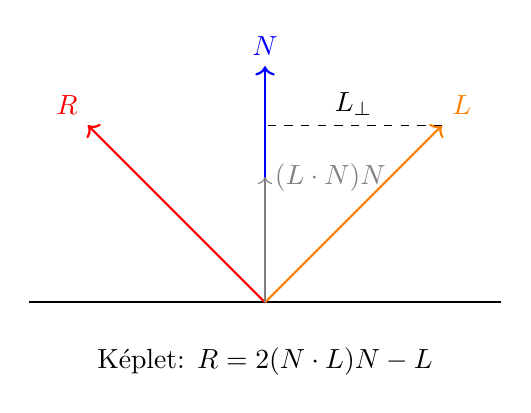
\begin{tikzpicture}[scale=1.5]
    \coordinate (O) at (0,0);
    \draw[thick] (-2,0) -- (2,0);
    \draw[->, thick, blue] (0,0) -- (0,2) node[above] {$N$};
    \draw[->, thick, orange] (0,0) -- (1.5, 1.5) node[above right] {$L$};
    \draw[->, thick, red] (0,0) -- (-1.5, 1.5) node[above left] {$R$};
    
    % Projection lines
    \draw[dashed] (1.5, 1.5) -- (0, 1.5) node[midway, above] {$L_{\perp}$};
    \draw[->, gray] (0,0) -- (0, 1.06) node[right] {$(L \cdot N)N$};
    
    \node at (0, -0.5) {Képlet: $R = 2(N \cdot L)N - L$};
\end{tikzpicture}
\end{center}

\subsection{Phong-modell kitevője ($n$)}
A $(R \cdot V)^n$ tagban az $n$ a felület simaságát (shininess) jellemzi.

\subsection{Árnyalási Interpoláció (Gouraud vs Phong)}
\begin{itemize}
    \item \textbf{Gouraud:} A színeket ($C$) interpoláljuk.
    $$ C_P = \alpha C_A + \beta C_B + \gamma C_C $$
    \item \textbf{Phong:} A normálvektorokat ($N$) interpoláljuk, majd minden pixelben újra normalizáljuk.
\end{itemize}

\section{Textúrázás}

A textúrázás során egy 2D-s képet (textúrát) feszítünk rá a 3D-s modellre.

\begin{center}
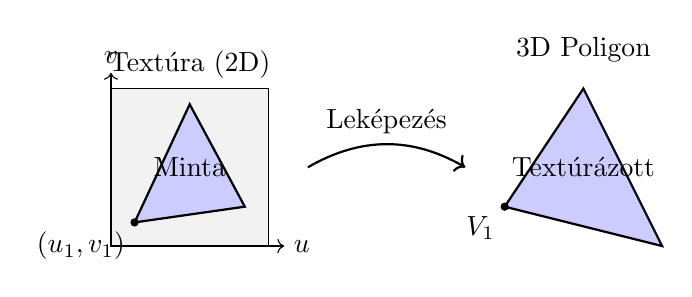
\begin{tikzpicture}
    % Texture
    \begin{scope}
        \draw[fill=gray!10] (0,0) rectangle (2,2);
        \node at (1,2.3) {Textúra (2D)};
        \draw[->] (0,0) -- (2.2,0) node[right] {$u$};
        \draw[->] (0,0) -- (0,2.2) node[above] {$v$};
        
        % Texture Triangle
        \coordinate (T1) at (0.3, 0.3);
        \coordinate (T2) at (1.7, 0.5);
        \coordinate (T3) at (1.0, 1.8);
        
        \draw[thick, fill=blue!20] (T1) -- (T2) -- (T3) -- cycle;
        \node at (1,1) {Minta};
        \fill (T1) circle (1.5pt) node[below left] {$(u_1, v_1)$};
    \end{scope}
    
    % Mapping Arrow
    \draw[->, thick, bend left] (2.5, 1) to node[above] {Leképezés} (4.5, 1);
    
    % 3D Object
    \begin{scope}[shift={(5,0.5)}]
        \node at (1,2) {3D Poligon};
        % 3D Triangle (projected)
        \coordinate (P1) at (0,0);
        \coordinate (P2) at (2,-0.5);
        \coordinate (P3) at (1, 1.5);
        
        \draw[thick, fill=blue!20] (P1) -- (P2) -- (P3) -- cycle;
        \fill (P1) circle (1.5pt) node[below left] {$V_1$};
        \node at (1, 0.5) {Textúrázott};
    \end{scope}
\end{tikzpicture}
\end{center}

\subsection{Perspektivikus korrekció}
Lineáris interpoláció a képernyő síkjában nem helyes.
Helyes eljárás: $u/w, v/w$ és $1/w$ interpolálása, majd osztás.


\end{document}